\documentclass[12pt,letterpaper]{article}
\usepackage{amssymb} %maths
\usepackage{amsmath} %maths
\usepackage{polynom}
\usepackage{graphicx}
\usepackage{pgfplots}
\usepackage{tikz}
\usepackage{caption}
\usepackage{subcaption}
\usepackage[margin=0.5in]{geometry}
\usepackage{multicol}
\usepackage{mhchem}
\usepackage{enumitem}

\usetikzlibrary{arrows.meta,angles,quotes}
\pagenumbering{gobble}
\graphicspath{{images/}}

\begin{document}
\noindent\textbf{Name: \hrulefill\quad Favorite Temperature: \hrulefill}    
\begin{center}
    \noindent\textit{Thermodynamics Take Home Quiz (Time Yourself and Complete the whole thing in 1 Hour 35 Minutes)}
\end{center}
\noindent \textbf{Multiple Choice (MCQ)}\hfill \underline{\textit{1 pt each}}
\begin{multicols*}{2}
    \begin{enumerate}
        \item Which plot represents an exothermic reaction? %[ZumdahlThermoDynamics.pdf Page 1, Question 2]
            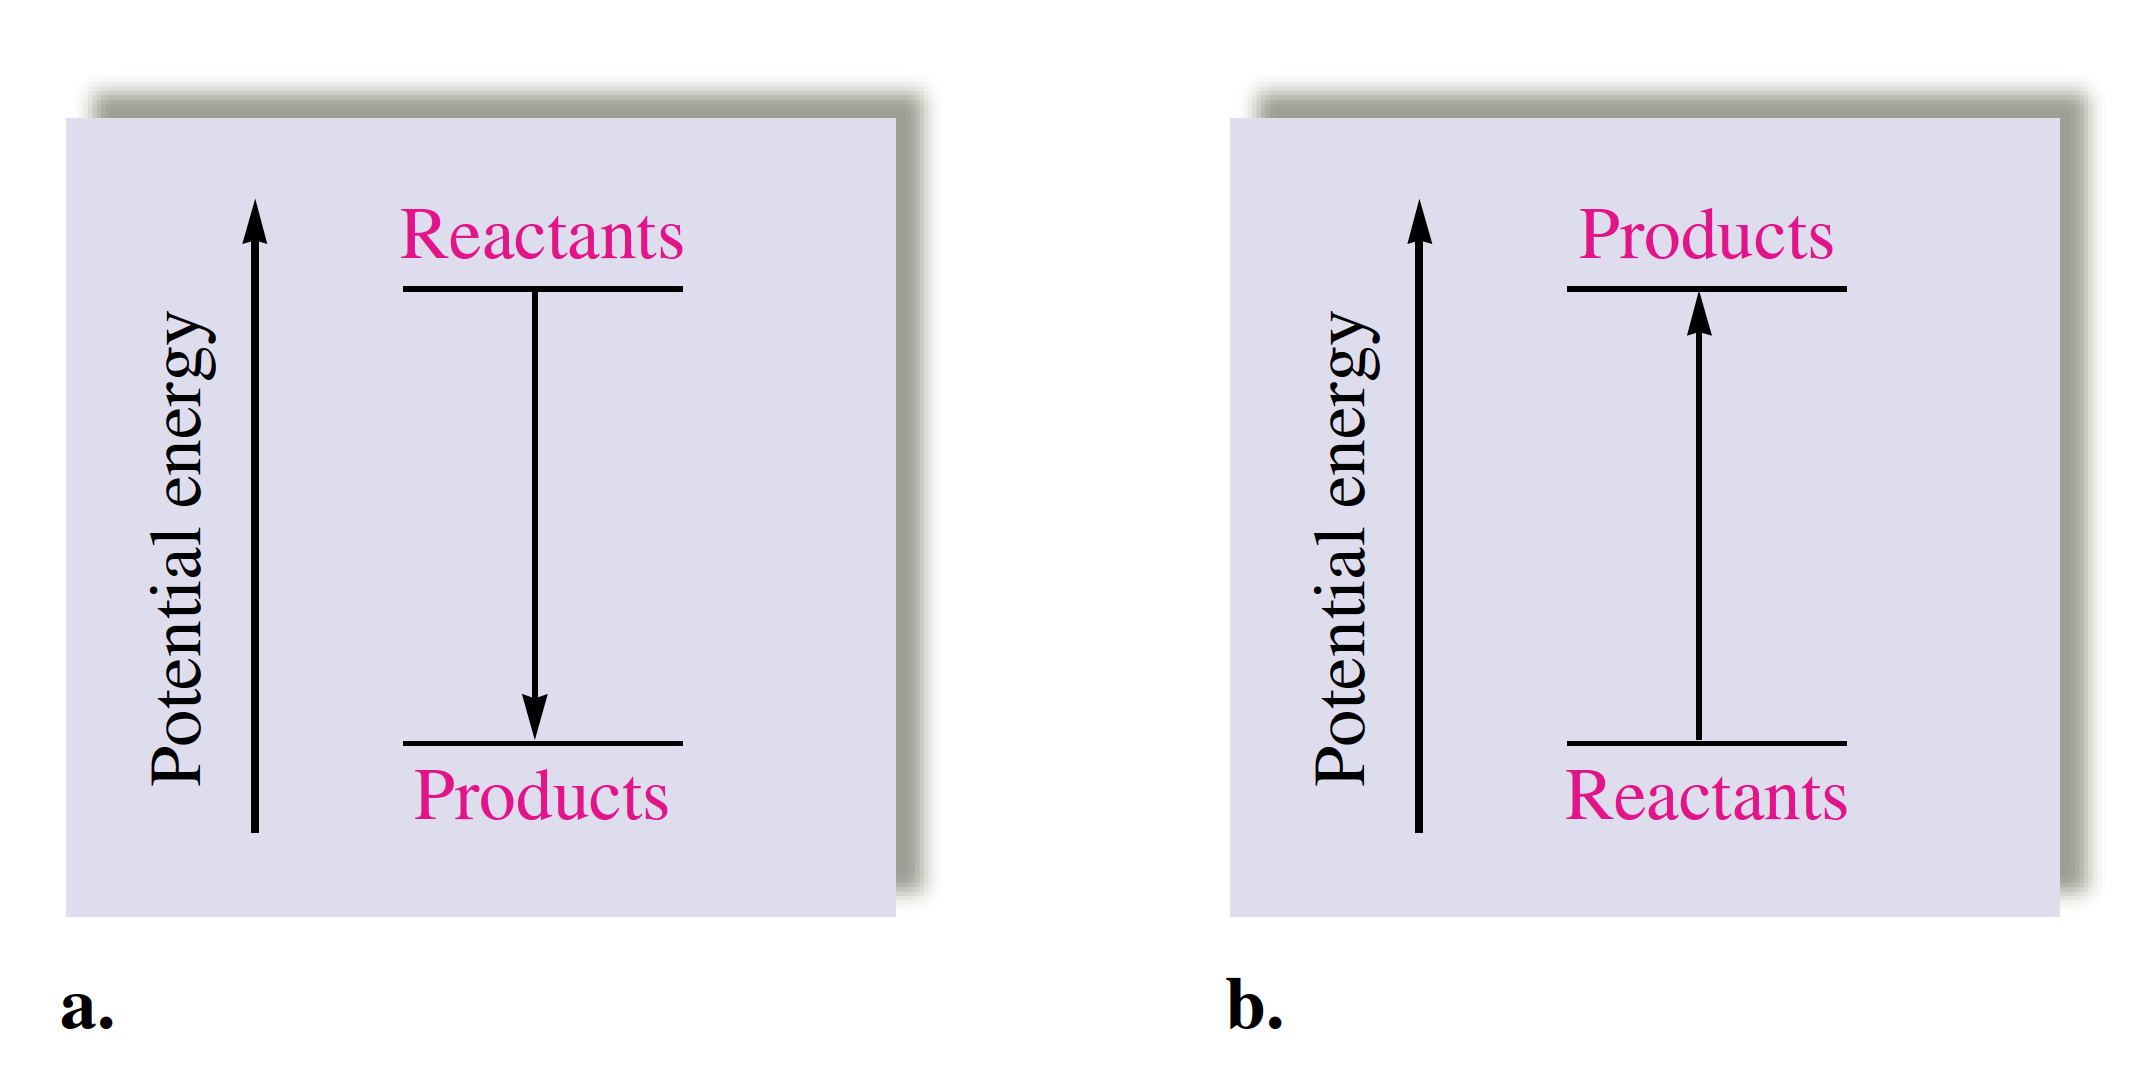
\includegraphics[width=\linewidth]{image1.png}
            \begin{enumerate}
                \item Plot a
                \item Plot b
                \item Both plot a and plot b
                \item Neither plot a nor plot b
            \end{enumerate}

        \item Calculate $\Delta E$ for a system that absorbs $82\text{ kJ}$ of heat and does $47\text{ kJ}$ of work. %[ZumdahlThermoDynamics.pdf Page 2, Question 21b]
            \begin{enumerate}
                \item $129\text{ kJ}$
                \item $35\text{ kJ}$
                \item $-35\text{ kJ}$
                \item $-129\text{ kJ}$
            \end{enumerate}

        \item One hundred joules of work are required to compress a gas. At the same time, the gas releases $23\text{ J}$ of heat. Calculate the internal energy change, $\Delta E$. %[ZumdahlThermoDynamics.pdf Page 3, Question 24a]
            \begin{enumerate}
                \item $+123\text{ J}$
                \item $-123\text{ J}$
                \item $-77\text{ J}$
                \item $+77\text{ J}$
            \end{enumerate}
        \columnbreak
        \item Consider the following reaction:
            \begin{equation*}
                \ce{2H2(g) + O2(g) -> 2H2O(l)} \quad \Delta H = -572\text{ kJ}
            \end{equation*}
            How much heat is evolved for the production of $1.00\text{ mol}$ of $\ce{H2O(l)}$? %[ZumdahlThermoDynamics.pdf Page 3, Question 36a]
            \begin{enumerate}
                \item $572\text{ kJ}$
                \item $1144\text{ kJ}$
                \item $286\text{ kJ}$
                \item $-286\text{ kJ}$
            \end{enumerate}

        \item The specific heat capacity of silver is $0.24\text{ J/}^\circ\text{C}\cdot\text{g}$. Calculate the energy required to raise the temperature of $150.0\text{ g}$ of $\ce{Ag}$ from $273\text{ K}$ to $298\text{ K}$. %[ZumdahlThermoDynamics.pdf Page 4, Question 42a]
            \begin{enumerate}
                \item $900\text{ J}$
                \item $9828\text{ J}$
                \item $10.7\text{ kJ}$
                \item $36\text{ J}$
            \end{enumerate}

        \item In a coffee-cup calorimeter, $50.0\text{ mL}$ of $0.100\text{ M}$ $\ce{AgNO3}$ and $50.0\text{ mL}$ of $0.100\text{ M}$ $\ce{HCl}$ are mixed. The temperature rises from $22.60\text{}^\circ\text{C}$ to $23.40\text{}^\circ\text{C}$. Calculate the heat ($\text{kJ/mol}$) for:
            \begin{equation*}
                \ce{Ag+(aq) + Cl-(aq) -> AgCl(s)}
            \end{equation*}
            (Assume $100.0\text{ g}$ solution, $C_p = 4.18\text{ J/}^\circ\text{C}\cdot\text{g}$). %[ZumdahlThermoDynamics.pdf Page 4, Question 51]
            \begin{enumerate}
                \item $-66\text{ kJ/mol}$
                \item $+66\text{ kJ/mol}$
                \item $-334\text{ kJ/mol}$
                \item $-0.334\text{ kJ/mol}$
            \end{enumerate}
        \columnbreak
        \item Calculate $\Delta H$ for the reaction:
            \begin{equation*}
                \ce{2C(s) + O2(g) -> 2CO(g)}
            \end{equation*}
            Given: $\ce{C(s) + O2(g) -> CO2(g)}$ $\Delta H = -393.7\text{ kJ/mol}$ and $\ce{CO(g) + 1/2O2(g) -> CO2(g)}$ $\Delta H = -283.3\text{ kJ/mol}$. %[ZumdahlThermoDynamics.pdf Page 4, Question 57]
            \begin{enumerate}
                \item $-110.4\text{ kJ}$
                \item $-220.8\text{ kJ}$
                \item $-677.0\text{ kJ}$
                \item $+110.4\text{ kJ}$
            \end{enumerate}

        \item Which of the following reactions has $\Delta H^\circ$ values equal to $\Delta H_f^\circ$ for the product? %[ZumdahlThermoDynamics.pdf Page 5, Question 65]
            \begin{enumerate}
                \item $\ce{Na(s) + 1/2Cl2(g) -> NaCl(s)}$
                \item $\ce{Na(g) + 1/2Cl2(g) -> NaCl(s)}$
                \item $\ce{2Na(s) + Cl2(g) -> 2NaCl(s)}$
                \item $\ce{Na+(aq) + Cl-(aq) -> NaCl(s)}$
            \end{enumerate}

        \item For the process $\ce{H2O(l) -> H2O(g)}$ at $298\text{ K}$ and $1.0\text{ atm}$, $\Delta H$ is more positive than $\Delta E$ by $2.5\text{ kJ/mol}$. What does this $2.5\text{ kJ/mol}$ represent? %[ZumdahlThermoDynamics.pdf Page 4, Question 39]
            \begin{enumerate}
                \item Heat of fusion
                \item Work done by the system to push back the atmosphere
                \item Activation energy
                \item Entropy change
            \end{enumerate}
        \item Calculate the enthalpy change for the reaction:
            \begin{align*}
                &\ce{CH4(g) + 2O2(g) -> CO2(g) + 2H2O(l)}\\ 
                &\Delta H = -891\text{ kJ}
            \end{align*}
            When $1.00\text{ g}$ of methane is burned in excess oxygen. %[ZumdahlThermoDynamics.pdf Page 3, Question 38a]
            \begin{enumerate}
                \item $-891\text{ kJ}$
                \item $-55.7\text{ kJ}$
                \item $-14.3\text{ kJ}$
                \item $+55.7\text{ kJ}$
            \end{enumerate}
        \columnbreak
        \item Predict the sign of $\Delta S_{surr}$ for the process: $\ce{H2O(l) -> H2O(g)}$. %[ZumdahlThermoDynamics.pdf Page 11, Question 25a]
            \begin{enumerate}
                \item Positive
                \item Negative
                \item Zero
                \item Depends on the temperature
            \end{enumerate}

        \item Calculate $\Delta S_{surr}$ for the following reaction at $25\text{}^\circ\text{C}$ and $1\text{ atm}$:
            \begin{align*}
                &\ce{C3H8(g) + 5O2(g) -> 3CO2(g) + 4H2O(l)}\\
                &\Delta H^\circ = -2221\text{ kJ}
            \end{align*}
            %[ZumdahlThermoDynamics.pdf Page 12, Question 26a]
            \begin{enumerate}
                \item $7.45\text{ J/K}$
                \item $7450\text{ J/K}$
                \item $-7450\text{ J/K}$
                \item $89.3\text{ J/K}$
            \end{enumerate}

        \item For mercury, the enthalpy of vaporization is $58.51\text{ kJ/mol}$ and the entropy of vaporization is $92.92\text{ J/K}\cdot\text{mol}$. What is the normal boiling point of mercury? %[ZumdahlThermoDynamics.pdf Page 12, Question 30]
            \begin{enumerate}
                \item $0.630\text{ K}$
                \item $630\text{ K}$
                \item $357\text{ K}$
                \item $630\text{}^\circ\text{C}$
            \end{enumerate}

        \item Predict the sign of $\Delta S^\circ$ for the following reaction:
            \begin{equation*}
                \ce{2H2(g) + O2(g) -> 2H2O(l)}
            \end{equation*}
            %[ZumdahlThermoDynamics.pdf Page 12, Question 33c]
            \begin{enumerate}
                \item Positive
                \item Negative
                \item Zero
                \item Cannot be predicted
            \end{enumerate}

        \item Which substance has the greater value of $S^\circ$? %[ZumdahlThermoDynamics.pdf Page 12, Question 35b]
            \begin{enumerate}
                \item $\ce{C2H5OH(l)}$
                \item $\ce{C2H5OH(g)}$
                \item Both are equal
                \item $\ce{C2H5OH(s)}$
            \end{enumerate}
        \columnbreak
        \item Calculate $\Delta G^\circ$ for the reaction:
            \begin{equation*}
                \ce{2NO2(g) <=> N2O4(g)}
            \end{equation*}
            Given $\Delta H^\circ = -58.03\text{ kJ}$ and $\Delta S^\circ = -176.6\text{ J/K}$ at $298\text{ K}$. %[ZumdahlThermoDynamics.pdf Page 13, Question 47]
            \begin{enumerate}
                \item $-5.40\text{ kJ}$
                \item $-110.6\text{ kJ}$
                \item $+5.40\text{ kJ}$
                \item $-58.2\text{ kJ}$
            \end{enumerate}

        \item At what temperature is $\Delta G^\circ = 0$ for the reaction $\ce{2NO2(g) <=> N2O4(g)}$? (Assume $\Delta H^\circ = -58.03\text{ kJ}$ and $\Delta S^\circ = -176.6\text{ J/K}$). %[ZumdahlThermoDynamics.pdf Page 13, Question 47]
            \begin{enumerate}
                \item $0.328\text{ K}$
                \item $328.6\text{ K}$
                \item $298\text{ K}$
                \item $3.04\text{ K}$
            \end{enumerate}
        \item Using the equation $\Delta G^\circ = -RT\ln(K)$, calculate $\Delta G^\circ$ for a reaction with $K = 0.090$ at $25\text{}^\circ\text{C}$. %[ZumdahlThermoDynamics.pdf Page 15, Question 74a]
            \begin{enumerate}
                \item $6.0\text{ kJ}$
                \item $-6.0\text{ kJ}$
                \item $0.50\text{ kJ}$
                \item $22\text{ kJ}$
            \end{enumerate}

        \item Which of the following processes are spontaneous? %[ZumdahlThermoDynamics.pdf Page 11, Question 19]
            \begin{enumerate}
                \item Salt dissolves in $\ce{H2O}$
                \item Iron rusts
                \item A clear solution becomes uniform color after dye is added
                \item All of the above
            \end{enumerate}
        \columnbreak
        \item Calculate $\Delta S^\circ$ for the reaction:
            \begin{equation*}
                \ce{2H2S(g) + SO2(g) -> 3S_{rhombic}(s) + 2H2O(g)}
            \end{equation*}
            Given $S^\circ$ values ($\text{J/K}\cdot\text{mol}$): $\ce{H2S(g)} = 206$, $\ce{SO2(g)} = 248$, $\ce{S(s)} = 32$, $\ce{H2O(g)} = 189$. %[ZumdahlThermoDynamics.pdf Page 12, Question 37a]
            \begin{enumerate}
                \item $+186\text{ J/K}$
                \item $-186\text{ J/K}$
                \item $-474\text{ J/K}$
                \item $+474\text{ J/K}$
            \end{enumerate}

        \item In reaction 1, seven particles in solution form one particle. In reaction 2, four particles form one. Which reaction has a more favorable $\Delta S$? %[ZumdahlThermoDynamics.pdf Page 14, Question 81]
            \begin{enumerate}
                \item Reaction 1
                \item Reaction 2
                \item Both are equal
                \item Neither is favorable
            \end{enumerate}

        \item For an endothermic reaction, does the temperature of the calorimeter increase or decrease? %[ZumdahlThermoDynamics.pdf Page 1, Question 7]
            \begin{enumerate}
                \item Increase
                \item Decrease
                \item Remain the same
                \item Increase then decrease
            \end{enumerate}

        \item If the internal energy of a thermodynamic system is increased by $300\text{. J}$ while $75\text{ J}$ of expansion work is done, how much heat was transferred? %[ZumdahlThermoDynamics.pdf Page 3, Question 23]
            \begin{enumerate}
                \item $225\text{ J}$
                \item $375\text{ J}$
                \item $-375\text{ J}$
                \item $-225\text{ J}$
            \end{enumerate}

        \item Which of the following represents an increase in entropy? %[Thermodynamics Multiple Choice May 2019.pdf Page 1, Question 1]
            \begin{enumerate}
                \item freezing of water
                \item boiling of water
                \item crystallization of salt
                \item $\ce{2NO(g) -> N2O2(g)}$
            \end{enumerate}

        \item Calculate the entropy change for methanol ($\ce{CH3OH}$) going from a liquid to vapor. ($\Delta H_{vap} = 35.3\text{ kJ/mol}$, $T_b = 64.2\text{}^\circ\text{C}$). %[Thermodynamics Multiple Choice May 2019.pdf Page 1, Question 2]
            \begin{enumerate}
                \item $600\text{ J/K}\cdot\text{mol}$
                \item $551\text{ J/K}\cdot\text{mol}$
                \item $105\text{ J/K}\cdot\text{mol}$
                \item $-105\text{ J/K}\cdot\text{mol}$
            \end{enumerate}
        \item Any irreversible process results in an overall increase in: %[Thermodynamics Multiple Choice May 2019.pdf Page 2, Question 7]
            \begin{enumerate}
                \item Entropy
                \item Enthalpy
                \item Free Energy
                \item Temperature
            \end{enumerate}
        \item $\Delta S^\circ$ is positive for the reaction: %[Thermodynamics Multiple Choice May 2019.pdf Page 3, Question 11]
            \begin{enumerate}
                \item $\ce{Pb(NO3)2(aq) + 2KI(aq) -> PbI2(s) + 2KNO3(aq)}$
                \item $\ce{2H2O(g) -> 2H2(g) + O2(g)}$
                \item $\ce{H2O(g) -> H2O(s)}$
                \item $\ce{NO(g) + O2(g) -> NO2(g)}$
            \end{enumerate}

        \item For a reaction to be spontaneous under standard conditions at all temperatures, the signs of $\Delta H^\circ$ and $\Delta S^\circ$ must be: %[Thermodynamics Multiple Choice May 2019.pdf Page 11, Question 38]
            \begin{enumerate}
                \item $+, +$
                \item $+, -$
                \item $-, +$
                \item $-, -$
            \end{enumerate}

        \item The equilibrium constant for a reaction is $0.48$ at $25\text{}^\circ\text{C}$. What is the value of $\Delta G^\circ$ ($\text{kJ/mol}$)? %[Thermodynamics Multiple Choice May 2019.pdf Page 9, Question 31]
            \begin{enumerate}
                \item $1.8\text{ kJ/mol}$
                \item $-4.2\text{ kJ/mol}$
                \item $1.5 \times 10^2\text{ kJ/mol}$
                \item $4.2\text{ kJ/mol}$
            \end{enumerate}
        \columnbreak
        \item For any reaction at equilibrium, which of the following is true? %[Thermodynamics Multiple Choice May 2019.pdf Page 15, Question 57]
            \begin{enumerate}
                \item $\Delta H < 0$
                \item $\Delta S = 0$
                \item $\Delta H = 0$
                \item $\Delta G = 0$
            \end{enumerate}

        \item Find the temperature (in $\text{K}$) above which a reaction with a $\Delta H^\circ$ of $53.0\text{ kJ/mol}$ and a $\Delta S^\circ$ of $100.00\text{ J/K}\cdot\text{mol}$ becomes spontaneous. %[Thermodynamics Multiple Choice May 2019.pdf Page 13, Question 47]
            \begin{enumerate}
                \item $530\text{ K}$
                \item $0.53\text{ K}$
                \item $100\text{ K}$
                \item $273\text{ K}$
            \end{enumerate}

        \item If a process is exothermic and not spontaneous, then what must be true? %[Thermodynamics Multiple Choice May 2019.pdf Page 14, Question 56]
            \begin{enumerate}
                \item $\Delta S > 0$
                \item $\Delta H > 0$
                \item $\Delta G = 0$
                \item $\Delta S < 0$
            \end{enumerate}

        \item When ice melts at its normal melting point ($273.16\text{ K}$, $1\text{ atm}$), which of the following is true? %[Thermodynamics Multiple Choice May 2019.pdf Page 17, Question 8]
            \begin{enumerate}
                \item $\Delta H < 0, \Delta S > 0$
                \item $\Delta H > 0, \Delta S < 0$
                \item $\Delta H = 0, \Delta S = 0$
                \item $\Delta H > 0, \Delta S > 0$
            \end{enumerate}
    \end{enumerate}
\end{multicols*}
\pagebreak
\noindent \textbf{Free Response Questions (FRQ)}\hfill \underline{\textit{2 pts each}}
\begin{enumerate}
    \item A student investigates the reactions of nitrogen oxides. One of the reactions in the investigation requires an equimolar mixture of $\ce{NO(g)}$ and $\ce{NO2(g)}$, which the student produces by using the reaction represented below.
    \begin{equation*}
    \ce{2NO(g) + O2(g) -> 2NO2(g)}
    \end{equation*}
    
    \begin{enumerate}
        \item The particle-level representation of the equimolar mixture of $\ce{NO(g)}$ and $\ce{NO2(g)}$ in the flask at the completion of the reaction between $\ce{NO(g)}$ and $\ce{O2(g)}$ is shown below in the box on the right. In the box below on the left, draw the particle-level representation of the reactant mixture of $\ce{NO(g)}$ and $\ce{O2(g)}$ that would yield the product mixture shown in the box on the right. In your drawing, represent oxygen atoms and nitrogen atoms as indicated below.
        
        \begin{center}
        \begin{tabular}{|c|c|}
        \hline
        Oxygen atom = $\bigcirc$ & Nitrogen atom = $\bullet$ \\
        \hline
        \end{tabular}
        \end{center}
        
        \vspace{0.5cm}
        \begin{center}
        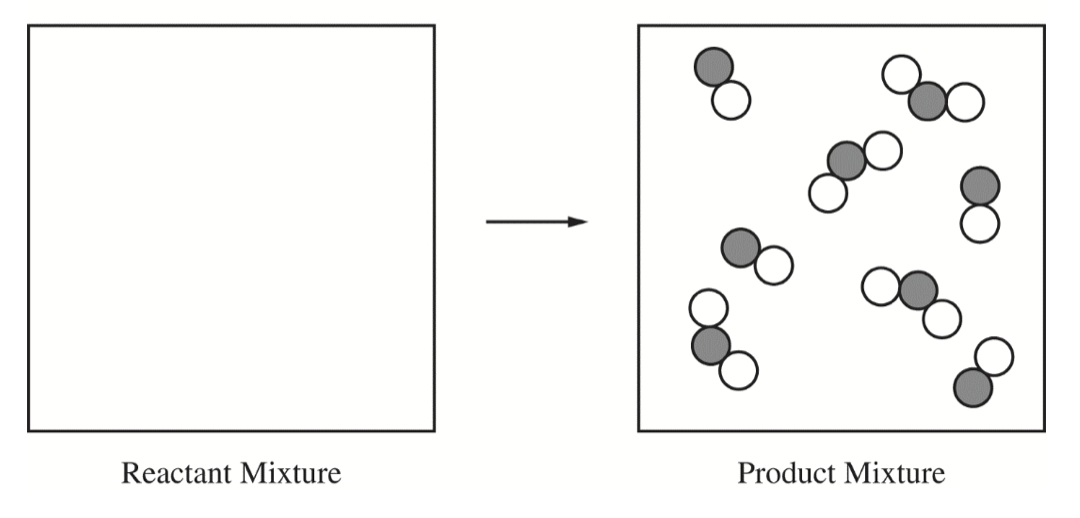
\includegraphics[width=0.6\textwidth]{image2.png}
        \end{center}
        
        The student reads in a reference text that $\ce{NO(g)}$ and $\ce{NO2(g)}$ will react as represented by the equation below. Thermodynamic data for the reaction are given in the table below the equation.
        
        \begin{equation*}
        \ce{NO(g) + NO2(g) <=> N2O3(g)}
        \end{equation*}
        
        \begin{center}
        \begin{tabular}{|c|c|c|}
        \hline
        $\Delta H_{298}$ & $\Delta S_{298}$ & $\Delta G_{298}$ \\
        \hline
        $-40.4\text{ kJ/mol}_{rxn}$ & $-138.5\text{ J/(K}\cdot\text{mol}_{rxn})$ & $0.87\text{ kJ/mol}_{rxn}$ \\
        \hline
        \end{tabular}
        \end{center}
        
        \item The student begins with an equimolar mixture of $\ce{NO(g)}$ and $\ce{NO2(g)}$ in a rigid reaction vessel and the mixture reaches equilibrium at $298\text{ K}$.
        \begin{enumerate}
            \item Calculate the value of the equilibrium constant, $K$, for the reaction at $298\text{ K}$.
            \item If both $P_{\ce{NO}}$ and $P_{\ce{NO2}}$ in the vessel are initially $1.0\text{ atm}$, will $P_{\ce{N2O3}}$ at equilibrium be equal to $1.0\text{ atm}$? Justify your answer.
        \end{enumerate}
        
        \item The student hypothesizes that increasing the temperature will increase the amount of $\ce{N2O3(g)}$ in the equilibrium mixture. Indicate whether you agree or disagree with the hypothesis. Justify your answer.
    \end{enumerate}
    \pagebreak
    \item A student performs a calorimetry experiment to determine the enthalpy of reaction for the dissolution of calcium carbonate in hydrochloric acid.
    
    \begin{equation*}
    \ce{CaCO3(s) + 2HCl(aq) -> CaCl2(aq) + CO2(g) + H2O(l)}
    \end{equation*}
    
    In order to measure the enthalpy of the reaction shown, the student repeats trial 1 by mixing $50.0\text{ mL}$ of $\ce{HCl(aq)}$ with $1.00\text{ g}$ of $\ce{CaCO3(s)}$ using a coffee cup calorimeter. The student records the temperature of the system every $20$ seconds. The data are given in the following table.
    
    \begin{center}
    \begin{tabular}{|c|c|}
    \hline
    Time (s) & \begin{tabular}{c} Measured Temperature of \\ Solution ($^\circ$C) \end{tabular} \\
    \hline
    0 & 21.20 \\
    \hline
    20 & 21.51 \\
    \hline  
    40 & 21.70 \\
    \hline
    60 & 21.85 \\
    \hline
    80 & 21.90 \\
    \hline
    100 & 21.90 \\
    \hline
    \end{tabular}
    \end{center}
    
    \begin{enumerate}
        \item Is the reaction endothermic or exothermic? Justify your answer using the information in the table.
        
        \item Based on the experimental data, the mass of the system is $51.0\text{ g}$, and the specific heat of the reaction mixture is $4.0\text{ J/(g}\cdot^\circ\text{C)}$.
        \begin{enumerate}
            \item Calculate the magnitude of heat transfer, $q$, in joules.
            \item Calculate the enthalpy of reaction in units of $\text{kJ/mol}_{rxn}$. Include the algebraic sign on your answer.
        \end{enumerate}
    \end{enumerate}
\end{enumerate}
\pagebreak
\section*{Answer Key}
\subsection*{Multiple Choice Answers:}
\begin{enumerate}
    \item \textbf{A} (Plot a). In an exothermic reaction, the products are lower in energy than the reactants. \textit{[Zumdahl Section 6, Page 265, Question 2]}
    
    \item \textbf{B} ($35\text{ kJ}$). Use $\Delta E = q + w$. Since $q = +82\text{ kJ}$ (absorbs) and $w = -47\text{ kJ}$ (does work), $\Delta E = 82 - 47 = 35\text{ kJ}$. \textit{[Zumdahl Section 6, Page 266, Question 21b]}
    
    \item \textbf{D} ($+77\text{ J}$). Use $\Delta E = q + w$. Here $w = +100\text{ J}$ (work on system) and $q = -23\text{ J}$ (heat released), so $\Delta E = 100 - 23 = 77\text{ J}$. \textit{[Zumdahl Section 6, Page 267, Question 24a]}
    
    \item \textbf{C} ($286\text{ kJ}$). The $\Delta H$ is for $2$ moles of \ce{H2O}. For $1$ mole, it is $572 / 2 = 286\text{ kJ}$. \textit{[Zumdahl Section 6, Page 267, Question 36a]}
    
    \item \textbf{A} ($900\text{ J}$). Use $q = mC\Delta T$. $q = (150.0\text{ g})(0.24\text{ J/g}\cdot^\circ\text{C})(298 - 273) = 900\text{ J}$. \textit{[Zumdahl Section 6, Page 268, Question 42a]}
    
    \item \textbf{A} ($-66\text{ kJ/mol}$). $q = mC\Delta T = 100 \cdot 4.18 \cdot 0.8 = 334.4\text{ J}$. Moles $= 0.050\text{ L} \cdot 0.100\text{ M} = 0.005\text{ mol}$. $\Delta H = -0.3344\text{ kJ} / 0.005\text{ mol} = -66.8\text{ kJ/mol}$. \textit{[Zumdahl Section 6, Page 268, Question 51]}
    
    \item \textbf{B} ($-220.8\text{ kJ}$). Multiply the first equation by $2$ and subtract $2$ times the second: $2(-393.7) - 2(-283.3) = -220.8\text{ kJ}$. \textit{[Zumdahl Section 6, Page 268, Question 57]}
    
    \item \textbf{A} (\ce{Na(s) + 1/2Cl2(g) -> NaCl(s)}). Enthalpy of formation requires elements in their standard states forming $1$ mole of product. \textit{[Zumdahl Section 6, Page 269, Question 65]}
    
    \item \textbf{B} (Work done by the system to push back the atmosphere). The difference between $\Delta H$ ($q_p$) and $\Delta E$ is $P\Delta V$, which is the work done against the atmosphere. \textit{[Zumdahl Section 6, Page 268, Question 39]}
    
    \item \textbf{B} ($-55.7\text{ kJ}$). Molar mass of \ce{CH4} $\approx 16\text{ g/mol}$. Heat $= (-891\text{ kJ/mol}) \times (1.00\text{ g}) / (16\text{ g/mol}) = -55.7\text{ kJ}$. \textit{[Zumdahl Section 6, Page 267, Question 38a]}
    
    \item \textbf{B} (Negative). $\Delta S_{surr} = -\Delta H / T$. Since vaporization is endothermic ($+\Delta H$), $\Delta S_{surr}$ is negative. \textit{[Zumdahl Section 16, Page 783, Question 25a]}
    
    \item \textbf{B} ($7450\text{ J/K}$). $\Delta S_{surr} = -\Delta H / T = -(-2221000\text{ J}) / 298\text{ K} = 7453\text{ J/K}$. \textit{[Zumdahl Section 16, Page 784, Question 26a]}
    
    \item \textbf{B} ($630\text{ K}$). At boiling point, $\Delta G = 0$, so $T = \Delta H / \Delta S = 58510 / 92.92 = 629.7\text{ K}$. \textit{[Zumdahl Section 16, Page 784, Question 30]}
    
    \item \textbf{B} (Negative). The reaction goes from $3$ moles of gas to liquid; entropy decreases significantly. \textit{[Zumdahl Section 16, Page 784, Question 33c]}
    
    \item \textbf{B} (\ce{C2H5OH(g)}). Gases have significantly higher entropy than liquids. \textit{[Zumdahl Section 16, Page 784, Question 35b]}
    
    \item \textbf{A} ($-5.40\text{ kJ}$). $\Delta G = \Delta H - T\Delta S = -58.03 - (298 \times -0.1766) = -5.40\text{ kJ}$. \textit{[Zumdahl Section 16, Page 785, Question 47]}
    
    \item \textbf{B} ($328.6\text{ K}$). $T = \Delta H / \Delta S = -58.03 / -0.1766 = 328.6\text{ K}$. \textit{[Zumdahl Section 16, Page 785, Question 47]}
    
    \item \textbf{A} ($6.0\text{ kJ}$). $\Delta G^\circ = -RT\ln(K) = -(8.314 \times 10^{-3} \times 298 \times \ln(0.090)) \approx 5.96\text{ kJ}$. \textit{[Zumdahl Section 16, Page 787, Question 74a]}
    
    \item \textbf{D} (All of the above). These are classic examples of spontaneous processes. \textit{[Zumdahl Section 16, Page 783, Question 19]}
    
    \item \textbf{B} ($-186\text{ J/K}$). $\Delta S = \Sigma S_{prod} - \Sigma S_{react} = (3 \times 32 + 2 \times 189) - (2 \times 206 + 248) = 474 - 660 = -186\text{ J/K}$. \textit{[Zumdahl Section 16, Page 784, Question 37a]}
    
    \item \textbf{B} (Reaction 2). A smaller decrease in disorder (fewer particles lost) results in a more favorable entropy. \textit{[Zumdahl Section 16, Page 786, Question 81]}
    
    \item \textbf{B} (Decrease). The system absorbs heat from the calorimeter, causing the calorimeter's temperature to drop. \textit{[Zumdahl Section 6, Page 265, Question 7]}
    
    \item \textbf{B} ($375\text{ J}$). $\Delta E = q + w \rightarrow 300 = q - 75 \rightarrow q = 375\text{ J}$. \textit{[Zumdahl Section 6, Page 267, Question 23]}
    
    \item \textbf{B} (Boiling). Vaporization increases randomness/microstates. \textit{[New Jersey Center for Teaching and Learning, Page 1, Question 1]}
    
    \item \textbf{C} ($105\text{ J/K}\cdot\text{mol}$). $\Delta S = \Delta H / T = 35300\text{ J} / (64.2 + 273.15)\text{ K} \approx 104.6\text{ J/K}\cdot\text{mol}$. \textit{[New Jersey Center for Teaching and Learning, Page 1, Question 2]}
    
    \item \textbf{A} (Entropy). Defined by the Second Law of Thermodynamics. \textit{[New Jersey Center for Teaching and Learning, Page 2, Question 7]}
    
    \item \textbf{B} (\ce{2H2O(g) -> 2H2(g) + O2(g)}). Increasing the number of moles of gas increases entropy. \textit{[New Jersey Center for Teaching and Learning, Page 3, Question 11]}
    
    \item \textbf{C} ($-, +$). Exothermic and increasing entropy is spontaneous at all temperatures. \textit{[New Jersey Center for Teaching and Learning, Page 11, Question 38]}
    
    \item \textbf{A} ($1.8\text{ kJ/mol}$). $\Delta G^\circ = -RT\ln(K) = -8.314 \times 298 \times \ln(0.48) \approx 1818\text{ J} = 1.8\text{ kJ}$. \textit{[New Jersey Center for Teaching and Learning, Page 9, Question 31]}
    
    \item \textbf{D} ($0$). By definition of equilibrium. \textit{[New Jersey Center for Teaching and Learning, Page 15, Question 57]}
    
    \item \textbf{A} ($530\text{ K}$). $T = \Delta H / \Delta S = 53000 / 100 = 530\text{ K}$. \textit{[New Jersey Center for Teaching and Learning, Page 13, Question 47]}
    
    \item \textbf{D} ($\Delta S < 0$). For an exothermic reaction ($-\Delta H$) to be non-spontaneous ($+\Delta G$), $\Delta S$ must be negative. \textit{[New Jersey Center for Teaching and Learning, Page 14, Question 56]}
    
    \item \textbf{D} ($\Delta H > 0, \Delta S > 0$). Melting is endothermic and increases disorder. \textit{[New Jersey Center for Teaching and Learning, Page 17, Question 8]}
\end{enumerate}

\subsection*{Free Response Answers}

\noindent \textbf{Question 1 (Nitrogen Oxides):} \textit{[2018 AP Chemistry FRQ, Question 2]}
\begin{enumerate}[label=(\alph*)]
    \item \textbf{(2 points total)}
    \begin{itemize}
        \item \textbf{1 point:} Correctly representing molecules of \ce{NO} and \ce{O2} in the reactant mixture
        \item \textbf{1 point:} Correctly representing atom conservation (8 molecules of \ce{NO} and 2 molecules of \ce{O2})
    \end{itemize}
    
    \item 
    \begin{enumerate}[label=(\roman*)]
        \item \textbf{(1 point)} Calculate equilibrium constant:
        
        $K = e^{-\Delta G^\circ/RT} = e^{-\frac{870\text{ J/mol}}{(8.314\text{ J/mol}\cdot\text{K})(298\text{ K})}} = e^{-0.351} = 0.70$
        
        \item \textbf{(1 point)} No, the pressure will not equal $1.0\text{ atm}$.
        
        $P_{\ce{N2O3}}$ would only equal $1.0\text{ atm}$ if the reaction goes to completion.
        
        \textbf{OR}
        
        The value of $K$ indicates that a substantial amount of reactants will be present at equilibrium.
    \end{enumerate}
    
    \item \textbf{(1 point)} Disagree.
    
    Because the reaction is exothermic, increasing the temperature of the reaction will favor the formation of the reactants (according to Le Ch\^atelier's principle).
\end{enumerate}

\noindent \textbf{Question 2 (Calorimetry):} \textit{[2023 AP Chemistry FRQ, Question 3]}
\begin{enumerate}[label=(\alph*)]
    \item \textbf{(1 point)} Exothermic. The solution temperature increases as the reaction proceeds.
    
    \item 
    \begin{enumerate}[label=(\roman*)]
        \item \textbf{(1 point)} Calculate heat transfer:
        
        $q_{surr} = mc\Delta T = (51.0\text{ g})(4.0\text{ J/g}\cdot^\circ\text{C})(21.90^\circ\text{C} - 21.20^\circ\text{C}) = 140\text{ J}$
        
        \item \textbf{(1 point)} Calculate enthalpy of reaction:
        
        $q_{sys} = -q_{surr} = -140\text{ J} = -0.14\text{ kJ}$
        
        $1.00\text{ g }\ce{CaCO3} \times \frac{1\text{ mol }\ce{CaCO3}}{100.09\text{ g }\ce{CaCO3}} \times \frac{1\text{ mol}_{rxn}}{1\text{ mol }\ce{CaCO3}} = 0.00999\text{ mol}_{rxn}$
        
        $\Delta H_{rxn} = \frac{-0.14\text{ kJ}}{0.00999\text{ mol}_{rxn}} = -14\text{ kJ/mol}_{rxn}$
    \end{enumerate}
\end{enumerate}
\end{document}